
\section{Quantum Chromodynamics and the Standard Model}
\label{qgp:qcd}

The Standard Model of Particle Physics is a highly descriptive quantum field theory that describes fundamental particle interactions.
The model predicts the existance of 17 distinct fundamental particles that make up all matter, anti-matter, and force carriers in the universe.
There are 3 generations of quarks and antiquarks, which are fermions that have color charge and participate in both the strong and electroweak interactions.
Then there are 3 generations of leptons and antileptons, which are also fermions, but only participate in electoweak interactions.
There are 4 vector gauge bosons: the photon which mediates the electromagnetic force, and the W and Z bosons which mediate the weak force, and the gluon which mediates the strong force.
Finally, there is a single scalar boson, which is the celebrated Higgs, discovered at the \gls{lhc} in 2008.

It explains the fundamental strong, weak, and electromagnetic interactions, which correspond to the group structure SU(3)$\times$SU(2)$\times$U(1).


Quantum chromodynamcs is the SU(3) part of the Standard Model that describes the strong interactions between colored quarks and gluons.

\begin{figure}[ht]
  \centering
  % Use .5\textwidth to only have the table fill half the page,
  % and \textwidth for the full page
  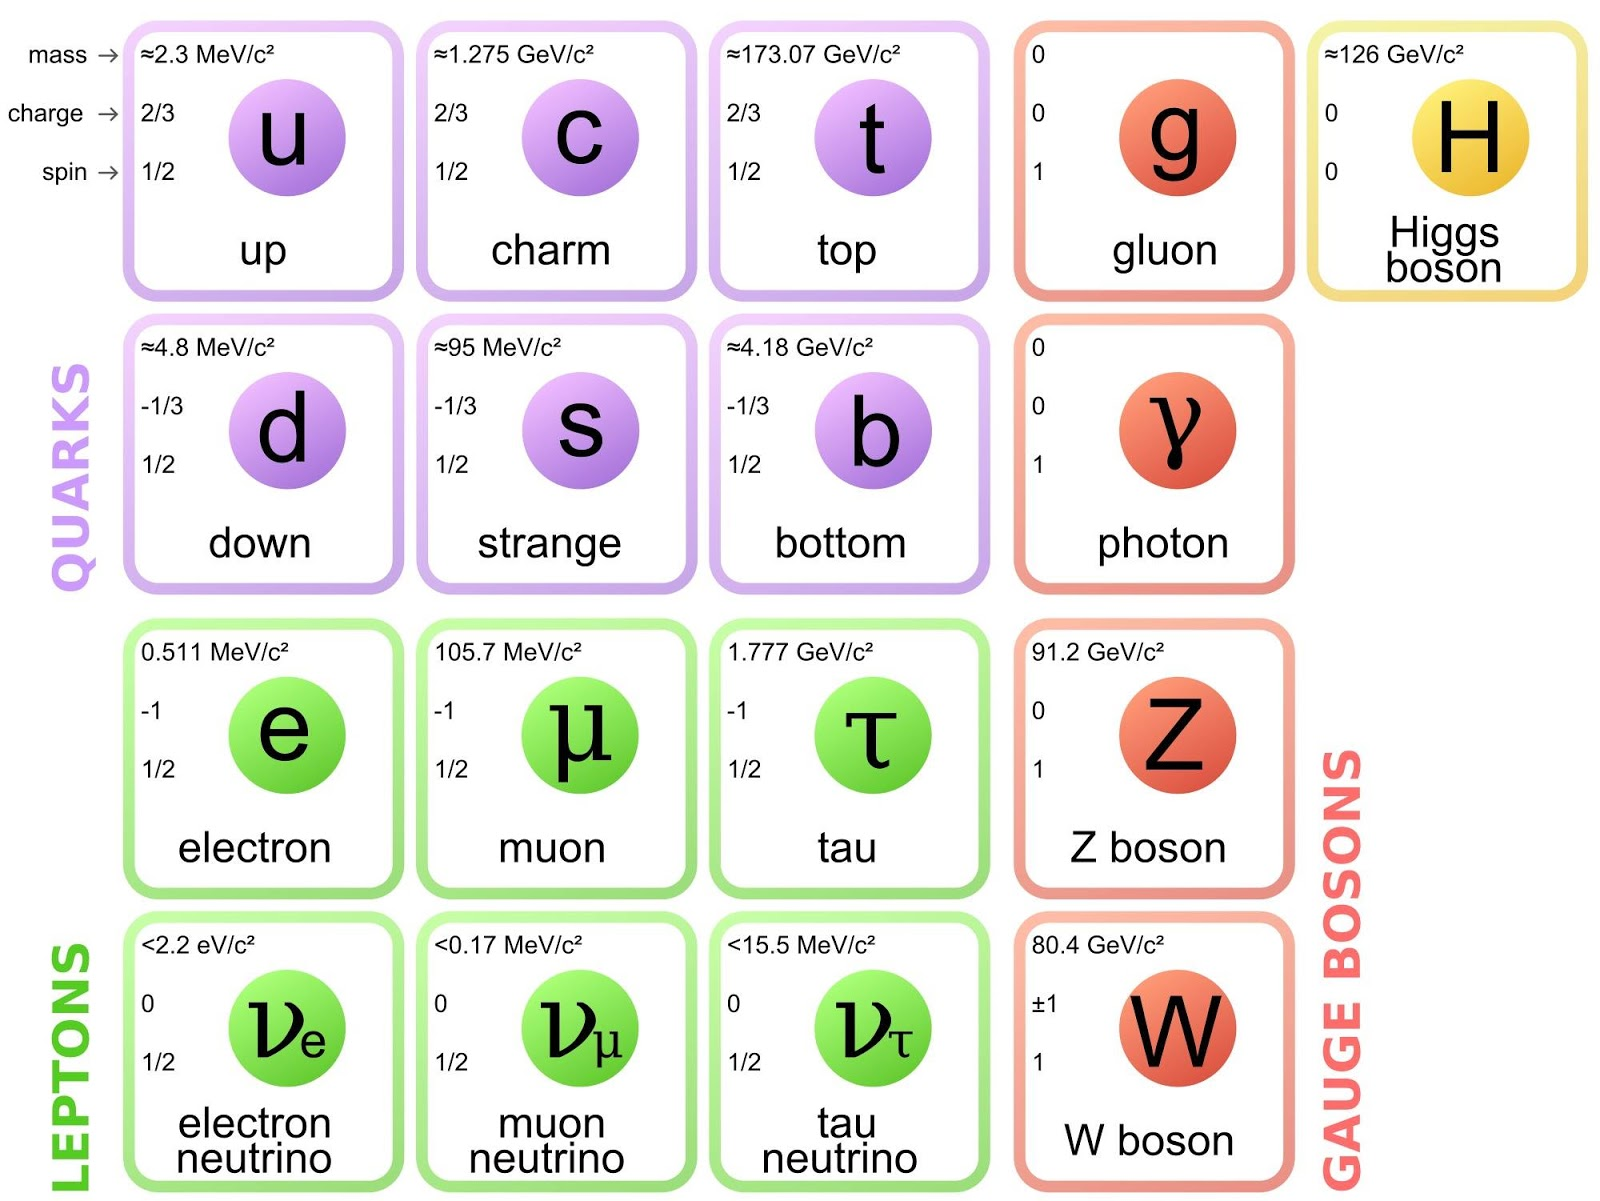
\includegraphics[width=.65\textwidth]{figures/standard-model.jpg}
  \caption{The fundamental particles posited by the Standard Model.}
  \label{fig:standard-model}
\end{figure}


The Lagrangian of QCD is given by
\begin{equation}
  \mathcal{L}_{\text{QCD}} = \sum_q \bar{\psi}_{q,a} \left( i\gamma^\mu \partial_\mu \delta_{ab} - g_s \gamma^\mu t_{ab}^{C} A_{\mu}^C - m_q \delta_{ab}\right)\psi_{q,b} - \frac{1}{4}F_{\mu\nu}^{A} F^{A\mu\nu}
\end{equation}
where pairs of indices are summed over and $\delta_{ab}$ is the Dirac-delta operator.
The $\gamma^\mu$ are the Dirac $\gamma$-matrices, which embed spin dynamics of fermions.
The $\psi_{q,a}$ are quark fields for a quark of flavor $q$, mass $m_q$, and color-index $a$ (which runs from 1 to 3).
The $A_\mu^C$ represent the gluon fields, with the index $C$ running from 1 to 8, meaning there are 8 types of gluons.
The $t_{ab}^C$ represent the generators of the SU(3) group, and correspond to 3$\times$3 matrices which embed the color dynamics on the quark/gluon interaction.
The quantity $g_s = \sqrt{4\pi\alpha_s}$ is the QCD coupling constant.
The gluon field tensor $F^{A}_{\mu\nu}$ is given by
\begin{equation}
  F_{\mu\nu}^A = \partial_\mu \mathcal{A}_\nu^A - \partial_\nu \mathcal{A}_\mu^A - g_s f_{ABC} \mathcal{A}_\mu^B \mathcal{A}_\mu^C
  \label{eqn:gluon-field-tensor}
\end{equation}
where $f_{ABC}$ are the structure constants of SU(3) and are defined by $[t^A,t^B] = if_{ABC}t^C$.
Note that the third term Eq. \ref{eqn:gluon-field-tensor} distinguishes QCD (the strong interaction), from QED (the electromagentic interaction).
This term gives rise to the triplet and quartic gluon self-interaction terms, which can be seen in the Feynman diagrams of QCD shown in Fig. \ref{fig:feynman-diagrams}.


\begin{figure}[ht]
  \begin{subfigure}{0.3\textwidth}
    \resizebox{\linewidth}{!}{
      \begin{tikzpicture}
        \begin{feynman}
          \vertex (a) {\( q \)};
          \vertex[below right=of a] (b);
          \vertex[below left=of b] (c) {\( q \)};
          \vertex[right=of b] (d) {\( g \)};
          \diagram*{
            (a) -- [fermion] (b),
            (b) -- [fermion] (c),
            (b) -- [gluon] (d),
          };
        \end{feynman}
      \end{tikzpicture}
    }
  \end{subfigure}
  \begin{subfigure}{0.3\textwidth}
    \resizebox{\linewidth}{!}{
      \begin{tikzpicture}
        \begin{feynman}
          \vertex (a) {\( g \)};
          \vertex[below right=of a] (b) ;
          \vertex[below left=of b] (c) {\( g \)};
          \vertex[right=of b] (d) {\( g \)};
          \diagram*{
            (a) -- [gluon] (b),
            (b) -- [gluon] (c),
            (b) -- [gluon] (d),
          };
        \end{feynman}
      \end{tikzpicture}
    }
  \end{subfigure}
  \begin{subfigure}{0.3\textwidth}
    \resizebox{\linewidth}{!}{
      \begin{tikzpicture}
      \begin{feynman}
        \vertex (a) {\( g \)};
        \vertex[below right=of a] (b) ;
        \vertex[below left=of b] (c) {\( g \)};
        \vertex[above right=of b] (d) {\( g \)};
        \vertex[below right=of b] (e) {\( g \)};
        \diagram*{
          (a) -- [gluon] (b),
          (b) -- [gluon] (c),
          (b) -- [gluon] (d),
          (b) -- [gluon] (e),
        };
      \end{feynman}
    \end{tikzpicture}
    }
  \end{subfigure}
  \caption{Feynman diagrams for the fundamental interaction vertices of QCD.}
  \label{fig:feynman-diagrams}
\end{figure}


Quarks and gluons are never observed in isolation, and instead always form into hadrons as color-neutral combinations of quarks, anti-quarks, and gluons.
This phenomena is known as \textit{color confinement}.
This occurs because, at low interaction energies, the strong force coupling (given by $g_s$, or, equivalently, $\alpha_s$) is strong.
The reason for this phenomena is not immediately intuitive, and stems from the renormalization scheme for $\alpha_s$.
The running coupling of the strong interaction strength $\alpha_s$ is derived from the renormlization group equation
\begin{equation}
  \label{eqn:RGE}
  Q^2 \cfrac{\partial \alpha_s}{\partial Q^2} = \beta(\alpha_s)
\end{equation}
where the QCD $\beta$-function has the following perturbative expansion:
\begin{equation}
  \label{eqn:beta-function}
  \beta(\alpha_s) = -b \alpha_s^2 \left[1 + b'\alpha_s + b''\alpha_s^2  + O(\alpha_s^3)\right]
\end{equation}
If we only keep the lowest order terms, Eq. \ref{eqn:RGE} becomes
\begin{equation}
  \label{eqn:RGE-lowest-order}
  Q^2 \cfrac{\partial \alpha_s}{\partial Q^2} \approx -b \alpha_s^2
\end{equation}
which has the solution
\begin{equation}
  \label{eqn:alpha-approx}
  \alpha_s \approx \cfrac{1}{b\ln\left(\frac{Q^2}{\Lambda^2}\right)}
\end{equation}
where $\Lambda$ comes from the choice of the constant of integration, and represents the scale at which the coupling will diverge.
While the exact value for $\Lambda$ is definition-dependent, it is often quoted as about 200 MeV.
Near the mass scale of light hadrons ($Q \sim 1$ GeV), $\alpha_s$ is large, which leads to the confinement of quarks and gluons inside hadrons.
As can be seen in \ref{eqn:alpha-approx}, high interaction energies (large $Q^2$), $\alpha_s$ becomes small.
This phenomena is known as \textit{asymptotic freedom}.
At high enough $Q^2$, quarks and gluons can be completely liberated from their hadronic bonds.

\begin{figure}[ht]
  \centering
  % Use .5\textwidth to only have the table fill half the page,
  % and \textwidth for the full page
  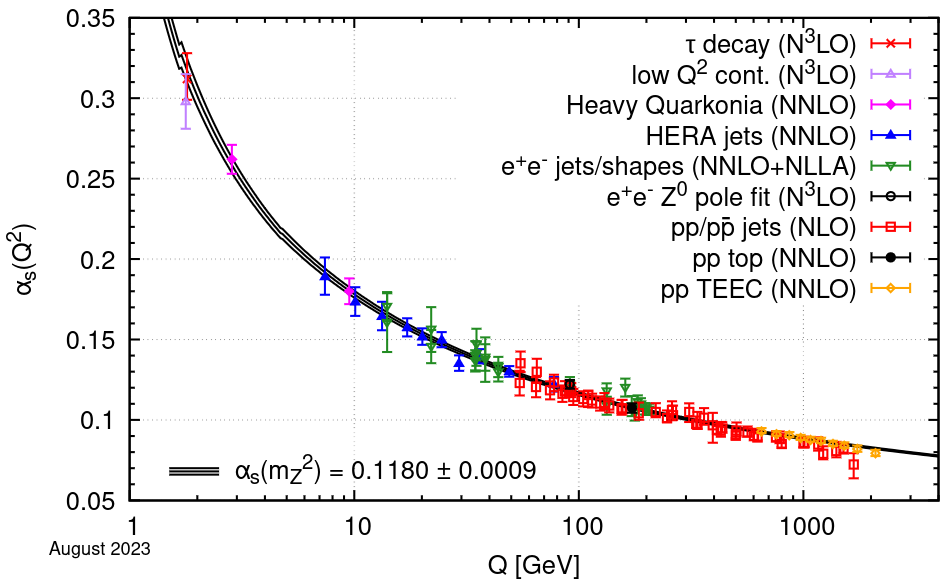
\includegraphics[width=.65\textwidth]{figures/running-coupling.png}
  \caption{Experimental measurements of the strong coupling strength $\alpha_s$ \protect\cite{ParticleDataGroup:2024cfk}.}
  \label{fig:running-coupling}
\end{figure}
%  Taken from \cite{ParticleDataGroup:2024cfk}









